\chapter{Functional Tests}\label{C:Functional-Tests}
Simultaneously with the development of IOSharp some small tests were created so the developed features could be tested to verify the properly operation of the implementation. There are three major tests without taking into account the simple GPIO. First of all an Arduino and a Raspberry Pi were connected through a Serial Port so the first one sends a message and the second replays again to the first. Secondly the SPI was tested using a RFID card reader and finally HomeSense gateway application was deployed on a Raspberry Pi.

\section{UART. Raspberry Pi and Netduino}\label{S:IOEx-UART}
This example shows that is possible to use the .NET Framework SerialPort implementation as a replacement of the original Micro Framework one. In this case a Raspberry Pi and a Netduino is used, the first one will send a message through the UART port, when the Netduino receives that message will send it back to the Raspberry Pi.
\begin{figure}[H]\begin{center}
 \centering
  \captionsetup{justification=centering}
  
\includegraphics[width=1\textwidth]{pictures/sample/red}
  \caption{Bytes exchanged between a Raspberry Pi and a Netduino using the UART \label{fig:IOEx-UART}}
\end{center}\end{figure}

The figure \ref{fig:IOEx-UART} shows the bytes sent through the \gls{TX} channel of the Raspberry Pi which are the same as the \gls{RX} connected to the Netduino.

\section{SPI. RFID and IOSharp}\label{S:rfid-iosharp}
This was the first test to verify the SPI in a real environment using a RFID card reader connected through the SPI bus. This test derives from a proof of concept made for VR gym in Argentona under the Spanish project "Activat" from "Proyecto Impacto", this project requested to develop a method to authenticate and authorize users for a secure entrance on a complex by using a RFID card reader and different cards, tags and wristbands with an ID which can be associated with a certain user.
\\
The project was developed using a Netduino Plus which uses Micro Framework and have interesting features such as network connectivity. The card reader used in this test is a MFRC522 chip from NXP which can use different communication protocols like SPI, UART and \gls{I2C}. But that chip is mounted on a MF522-AN board from Mifare which only offers a SPI interface. And this is the reason why this proof of concept was used to test the SPI feature.
\\
To communicate the Netduino with the card reader an API was written taking into account the MFRC522 datasheet (see on Appendix \ref{C:Libraries-Datasheets} the section \ref{SS:Libs-MFRC522-Datasheet}) and the existing Arduino implementation which uses Wiring, the Arduino programming language.
\\
The program creates an instance of this API and then starts the SPI configuration. Following this configuration a Timer is instantiated which will trigger a function at every certain time. This called function uses the API to communicate to the card reader and then retrieve the card ID if any is present after that it communicates again to obtain the Serial Number located in the card. Finally it prints this data in the console.

\subsection{Micro Framework version}\label{S:IOEx-SPI-Netduino}
The original example uses Micro Framework and the Secretlab classes for the Netduino Plus so the resulting binary will only work on this board. The port configuration for this example is really simple, because it only uses a pin for the \gls{CS}. The \gls{MOSI}, \gls{MISO} and \gls{SCLK} are defined by the board schema so the pins will be selected and configured internally on the virtual machine.

\begin{lstlisting}[language=CSharp, caption={SPIApi.cs - Configuring SPI for the MFRC522 in Netduino Plus}]
public void ConfigureSPI() {
    SPI.Configuration xSPIConfig;
    Cpu.Pin pin = Pins.GPIO_PIN_D9;

    xSPIConfig = new SPI.Configuration(pin, //Chip Select pin
        false, //Chip Select Active State
        50, //Chip Select Setup Time
        0, //Chip Select Hold Time
        false, //Clock Idle State
        true, //Clock Edge
        1000, //Clock Rate (kHz)
        SPI.SPI_module.SPI1); //SPI Module
    spiDevice = new SPI(xSPIConfig);
}
\end{lstlisting}
As it is shown above, the \gls{CS} pin is the \verb!Pins.GPIO_PIN_D9! which corresponds to a digital pin.

\subsection{Migrating to Linux}\label{S:IOEx-SPI-Migrating-to-IOSharp}
To use IOSharp instead of Micro Framework there is not a big requirement, basically the project must be converted to .NET Framework and then reference the IOSharp library, beside this library the mapping classes according to the deployment platform must also be referenced, in this case the Raspberry Pi pin library. The next step is change the pin for the \gls{CS} to the according one. Normally in Linux each SPI device have one or more \gls{CS} pins but not every pin is suitable to work with that SPI device, so it is important to check the appropriate pin.
\\
Taking in mind that using this test can also prove that IOSharp can work with the original code by doing a minimal set of changes it was tried to use one of the features that the Visual Studio projects offers. Declaring two solution files (\verb!*.sln!) which each one calls two different project files (\verb!*.csproj!) make possible to have one solution with the Micro Framework classes for the Netduino while the other one will contain the references for the IOSharp and the .NET Framework. This will create two different projects from the same code, one being able to run on Netduino and the other one in Linux.
\\
These were the major changes, and they cannot be considered real changes to the original code, because is possible to take the application program and create a new .NET Framework project with that code. Doing this changes is p a proof that is possible to maintain the same code for different platform deployments.
\\
Using conditional compiling is possible to set the required pin for each bord and each solution. In this case, the symbol used for the conditional compiling is \verb!MF! which is present on the Netduino version of the \verb!*.csproj! whereas the Raspberry Pi don't. Taking a look in the above code, for the Netduino the used pin is the \verb!Pins.GPIO_PIN_D9! and in the Raspberry Pi is \verb!Cpu.Pin.GPIO_Pin9!.

\begin{lstlisting}[language=CSharp, caption={SPIApi.cs - Conditional compiling symbol for NETMF and IOSharp}]
public void ConfigureSPI() {
    SPI.Configuration xSPIConfig;
    Cpu.Pin pin = Cpu.Pin.GPIO_NONE;
  	// In this case, the conditional compiling symbol used is MF, true for Micro Framework or false for IOSharp
  	#if MF
    	pin = Pins.GPIO_PIN_D9;
    #else
        pin = Cpu.Pin.GPIO_Pin9;
    #endif

    xSPIConfig = new SPI.Configuration(pin, //Chip Select pin
        false, //Chip Select Active State
        50, //Chip Select Setup Time
        0, //Chip Select Hold Time
        false, //Clock Idle State
        true, //Clock Edge
        1000, //Clock Rate (kHz)
        SPI.SPI_module.SPI1); //SPI Module
    spiDevice = new SPI(xSPIConfig);
    //MFRC522Init();
}
\end{lstlisting}

After doing this, this project can be opened as Micro Framework in order to deploy in a Netduino or open the Linux version. Deploying this application in any of these boards will result in a working program like the figure \ref{fig:IOEx-SPI} shows.
\begin{figure}[H]\begin{center}
 \centering
  \captionsetup{justification=centering}
  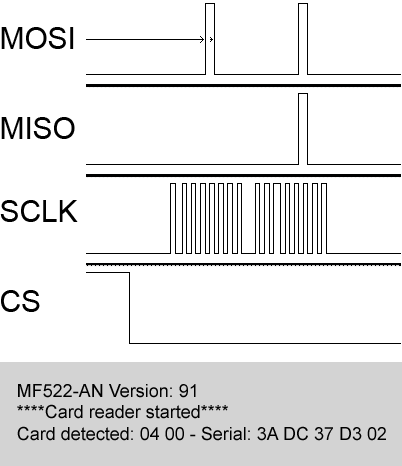
\includegraphics[width=0.5\textwidth]{pictures/examples/rfid-spi}
  \caption{Data exchange using the SPI\label{fig:IOEx-SPI}}
\end{center}\end{figure}

\section{HomeSense}\label{S:IOEx-HomeSense}
HomeSense is a Wireless Healthcare Sensor Platform designed by AlterAid. Its basis are the aim of control and care taking of the elderly and relatives. The current implementation uses a Netduino Mini which makes the function of the gateway which controls the sensor network, receiving all the data and uploading this to internet.
Some sensors are spread around the house which are capable of fetch     data, for example a sensor installed on the door of a medicine cabinet let the network know if that cabinet has been opened. So with all of this sensors is possible to acquire information from the environment and then send that information to the internet using the gateway.
\\
This sensors are programmed using C and all of them use the \gls{SoC} nRF24LE1 which mounts a low-power RF ISM band (2.4 GHz) from Nordic Semiconductor.
\begin{figure}[H]\begin{center}
 \centering
  \captionsetup{justification=centering}
  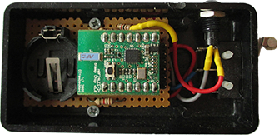
\includegraphics[scale=1]{pictures/examples/sensor}
  \caption{Sensor for a medicine cabinet\label{fig:IOEx-UART}}
\end{center}\end{figure}
The communication protocol designed for HomeSense is similar to a star network with multi-hop transmissions so it becomes a tree-start topology. The nodes try to fetch the gateway because this is on charge of upload the information to the internet.

\subsection{Gateway}\label{SS:IOEx-HomeSense-Gateway}
The program running on the gateway is programmed using Micro Framework and is deployed on a Netduino Mini. With IOSharp has been possible to deploy on a Raspberry Pi running Linux and Mono. The software running on the gateway controls the communication hardware and the mesh network using the designed protocol for this platform.
\\
Basically it will use all the features implemented in this library.

\begin{itemize}
\item \textbf{UART}: the Serial Port is used to transmit data between the Wifly and the Raspberry Pi. The Wifly is an XBee socket type module created by Roving Networks, and is used to connect to Wi-Fi networks. The communication between this module and the board where is connected is carried out using UART with a protocol described on the specification paper provided by the manufacturers.

\item \textbf{SPI}: The Nordic nRF24L01+ is controlled using the SPI protocol. This chip is used to create the physical meshed network which connects with the different nodes. The channel created using the Nordic is half-duplex so there is only one communication at a time either transmission or reception.
\item \textbf{Interruptions}: When the gateway's Nordic receives information form other nodes it must alert that new data is waiting to be read, to make this alert an interruption is used on a GPIO
\end{itemize}
With all this devices attached to the shield used in the Raspberry Pi will be possible to test all the functions working at the same time and how the system response compared to the original one.
\begin{figure}[H]\begin{center}
 \centering
  \captionsetup{justification=centering}
  \includegraphics[width=0.6\textwidth]{pictures/examples/raspihomestack}
  \caption{Raspberry Pi with the modules needed to run HomeSense\label{fig:IOEx-HS-Stack}}
\end{center}\end{figure}

\subsection{Working}\label{SS:IOEx-HomeSense-Working}
As IOSharp has implemented all the features required in HomeSense it is possible to change the project type from Micro Framework to .NET Framework and then reference this project. Finally the ports need to be remapped according to the shield used with the Raspberry Pi. The strategy to do this mapping is include the Hardware class of the Raspberry Pi and then rename the ports to the according ones. SerialPort device also must be renamed from \verb!COM1! to \verb!/dev/ttyAMA0!. After changing the references and the port names is possible to start testing the program. So it has been really easy to migrate from the Netduino Mini to the Raspberry Pi.
\\
\\
HomeSense has a program which shows the network status with its gateway and the different sensors connected to the network. On the following figure is shown the scenario. The aaaida logo represents the gateway whereas the node is represented by a door. In this case, both are linked as an arrow connects both of them. With this program is possible to know the network addresses of both devices. Also it shows other information like battery state or the fetched information by any sensor located on a node.
\begin{figure}[H]\begin{center}
 \centering
  \captionsetup{justification=centering}
  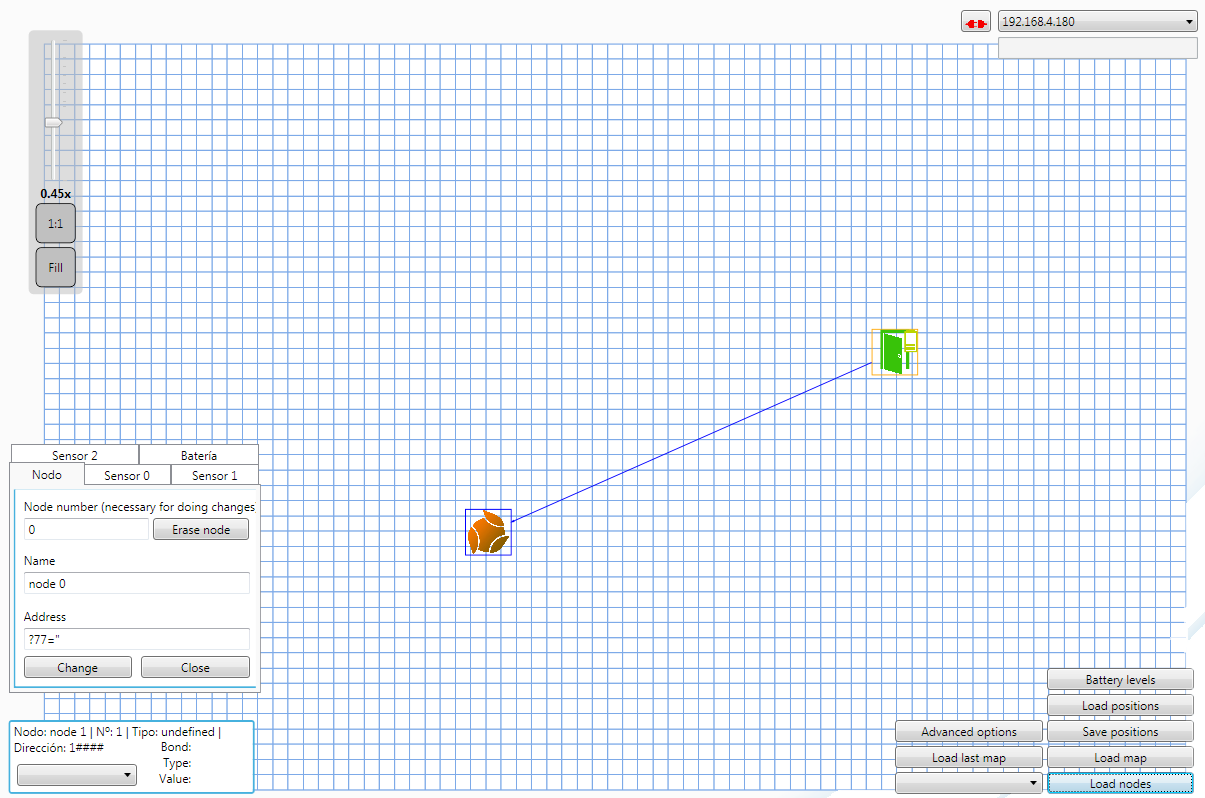
\includegraphics[width=1\textwidth]{pictures/examples/homesense-pillin}
  \caption{HomeSense dashboard. The aaaida logo on the left represents the Raspberry Pi (gateway)  whereas the door represents a sensor\label{fig:IOEx-HS-Dash}}
\end{center}\end{figure}

\section{Conclusions}\label{S:Results-overview}
After testing the different parts of IOSharp and deploying HomeSense on the Raspberry Pi using Mono it was seen that the performance was not as good as it was expected. Raspberry Pi, need more time to send the network events than the Netduino and this is probably related to the time needed to attend the interruptions on Mono. In this case the IOSharp with Mono needs two transmissions to send the same information that is send with only one transmission using the Netduino.
\\
To try to solve these issues with the performance of the library, IOSharp will be translated to C++ using a translating tool called AlterNative which is capable of translate .NET assemblies to C++ while maintaining a similar C\# syntax.